\section{Standard 1: Fair Comparison via Controlling Hyperparameter Volume}

\label{sec:nlp_benchmark_evals}

The first standard of our blueprint requires that empirical comparisons control for the volume of the hyperparameter search space. A common failure mode in machine learning resaerch occurs when a proposed method is heavily tuned while baselines are not. To operationalize this standard, we introduce the \textbf{``Best-of-N'' Evaluation Protocol}.
This protocol creates a fair comparison by equalizing the optimization effort: for any set of methods, we sample $N$ random hyperparameter configurations from preset hyperparameter spaces, and report the best performance achieved as a function of $N$, averaging over multiple random draws. This reveals whether a method is genuinely superior or simply benefits from a larger search budget.
The name is an allusion to ``Best-of-N'' sampling \citep{nakano2021webgpt,stiennon2020learning,hughes2024bestofnjailbreaking,schaeffer2025largelanguagemonkeyspower}, which is canonically used to obtain higher performance, and which we repurpose here as a generic evaluation protocol for fairly comparing any set of algorithms.


\begin{figure}[t!]
    \centering
    
\includegraphics[width=\linewidth]{figures/nlp_benchmark_evals/gsm8k_cot_llama/y=diff_of_em_strict_x=N_hue=sampler_row=model_col=task.pdf}
    \caption{\textbf{Applying the Best-of-N Protocol to GSM8K: \texttt{Min-p} Does Not Consistently Outperform Baselines.}
    In our second analysis, we measured how the difference between \texttt{min-p}'s highest score and the best non-\texttt{min-p} sampler's highest score changes as the number of swept hyperparameters increases. \texttt{Min-p} matches or underperforms other samplers.}
    \label{fig:gsm8k_diff_of_em_strict}
\end{figure}

\paragraph{Fair Comparison on NLP Benchmarks}

We applied this protocol to the claims made by \citet{nguyen2024minp}, which concluded that ``\texttt{Min-p} sampling achieves superior performance across benchmarks and temperatures.''
Verifying this claim required a computational effort significantly larger than the original study.
We used the authors' code to conduct an extensive sweep on GSM8K CoT \citep{cobbe2021gsm8k} totaling $\sim6000$ Nvidia A100-hours over the following models, samplers and hyperparameters:
%
\begin{itemize}
    \item \textbf{9 Models:} Qwen 2.5 \citep{qwen2025qwen25technicalreport} 0.5B, 1.5B, 3B and 7B; Mistral 7Bv0.1 \citep{jiang2023mistral7b}; Llama \citep{grattafiori2024llama3herdmodels} 3.1 8B and 3.2 3B; Gemma 2 \citep{gemmateam2024gemma2improvingopen} 2B and 9B.
    \item \textbf{2 Model Stages:} Pre-trained (``Base") and Post-Trained (``Instruct").
    \item \textbf{4 Samplers:} \texttt{basic}, \texttt{top-p}, \texttt{top-k}, \texttt{min-p}.
    \item \textbf{31 Temperatures:} $0.0$ (``greedy") to $3.0$ in increments of $0.1$.
    \item \textbf{6 Hyperparameters Per Sampler:} We chose $6$ hyperparameters per sampler, except for \texttt{basic} which has no hyperparameter beyond temperature. The values were taken from the original paper; some were lightly edited to make them more evenly distributed:
    \begin{itemize}
        \item \texttt{basic}: No hyperparameters other than temperature.
        \item \texttt{top-k}:  $k \in \{10, 30, 50, 100, 150, 200 \}$.
        \item \texttt{top-p}: $p \in \{0.99, 0.98, 0.95, 0.9, 0.8, 0.7 \}$.
        \item \texttt{min-p}: $p \in \{0.01, 0.02, 0.05, 0.1, 0.2, 0.3 \}$.
    \end{itemize}
    \item \textbf{3 Random Seeds for Sampling:} $\{0, 1, 2\}$
\end{itemize}


\begin{figure*}[t!]
    \centering
    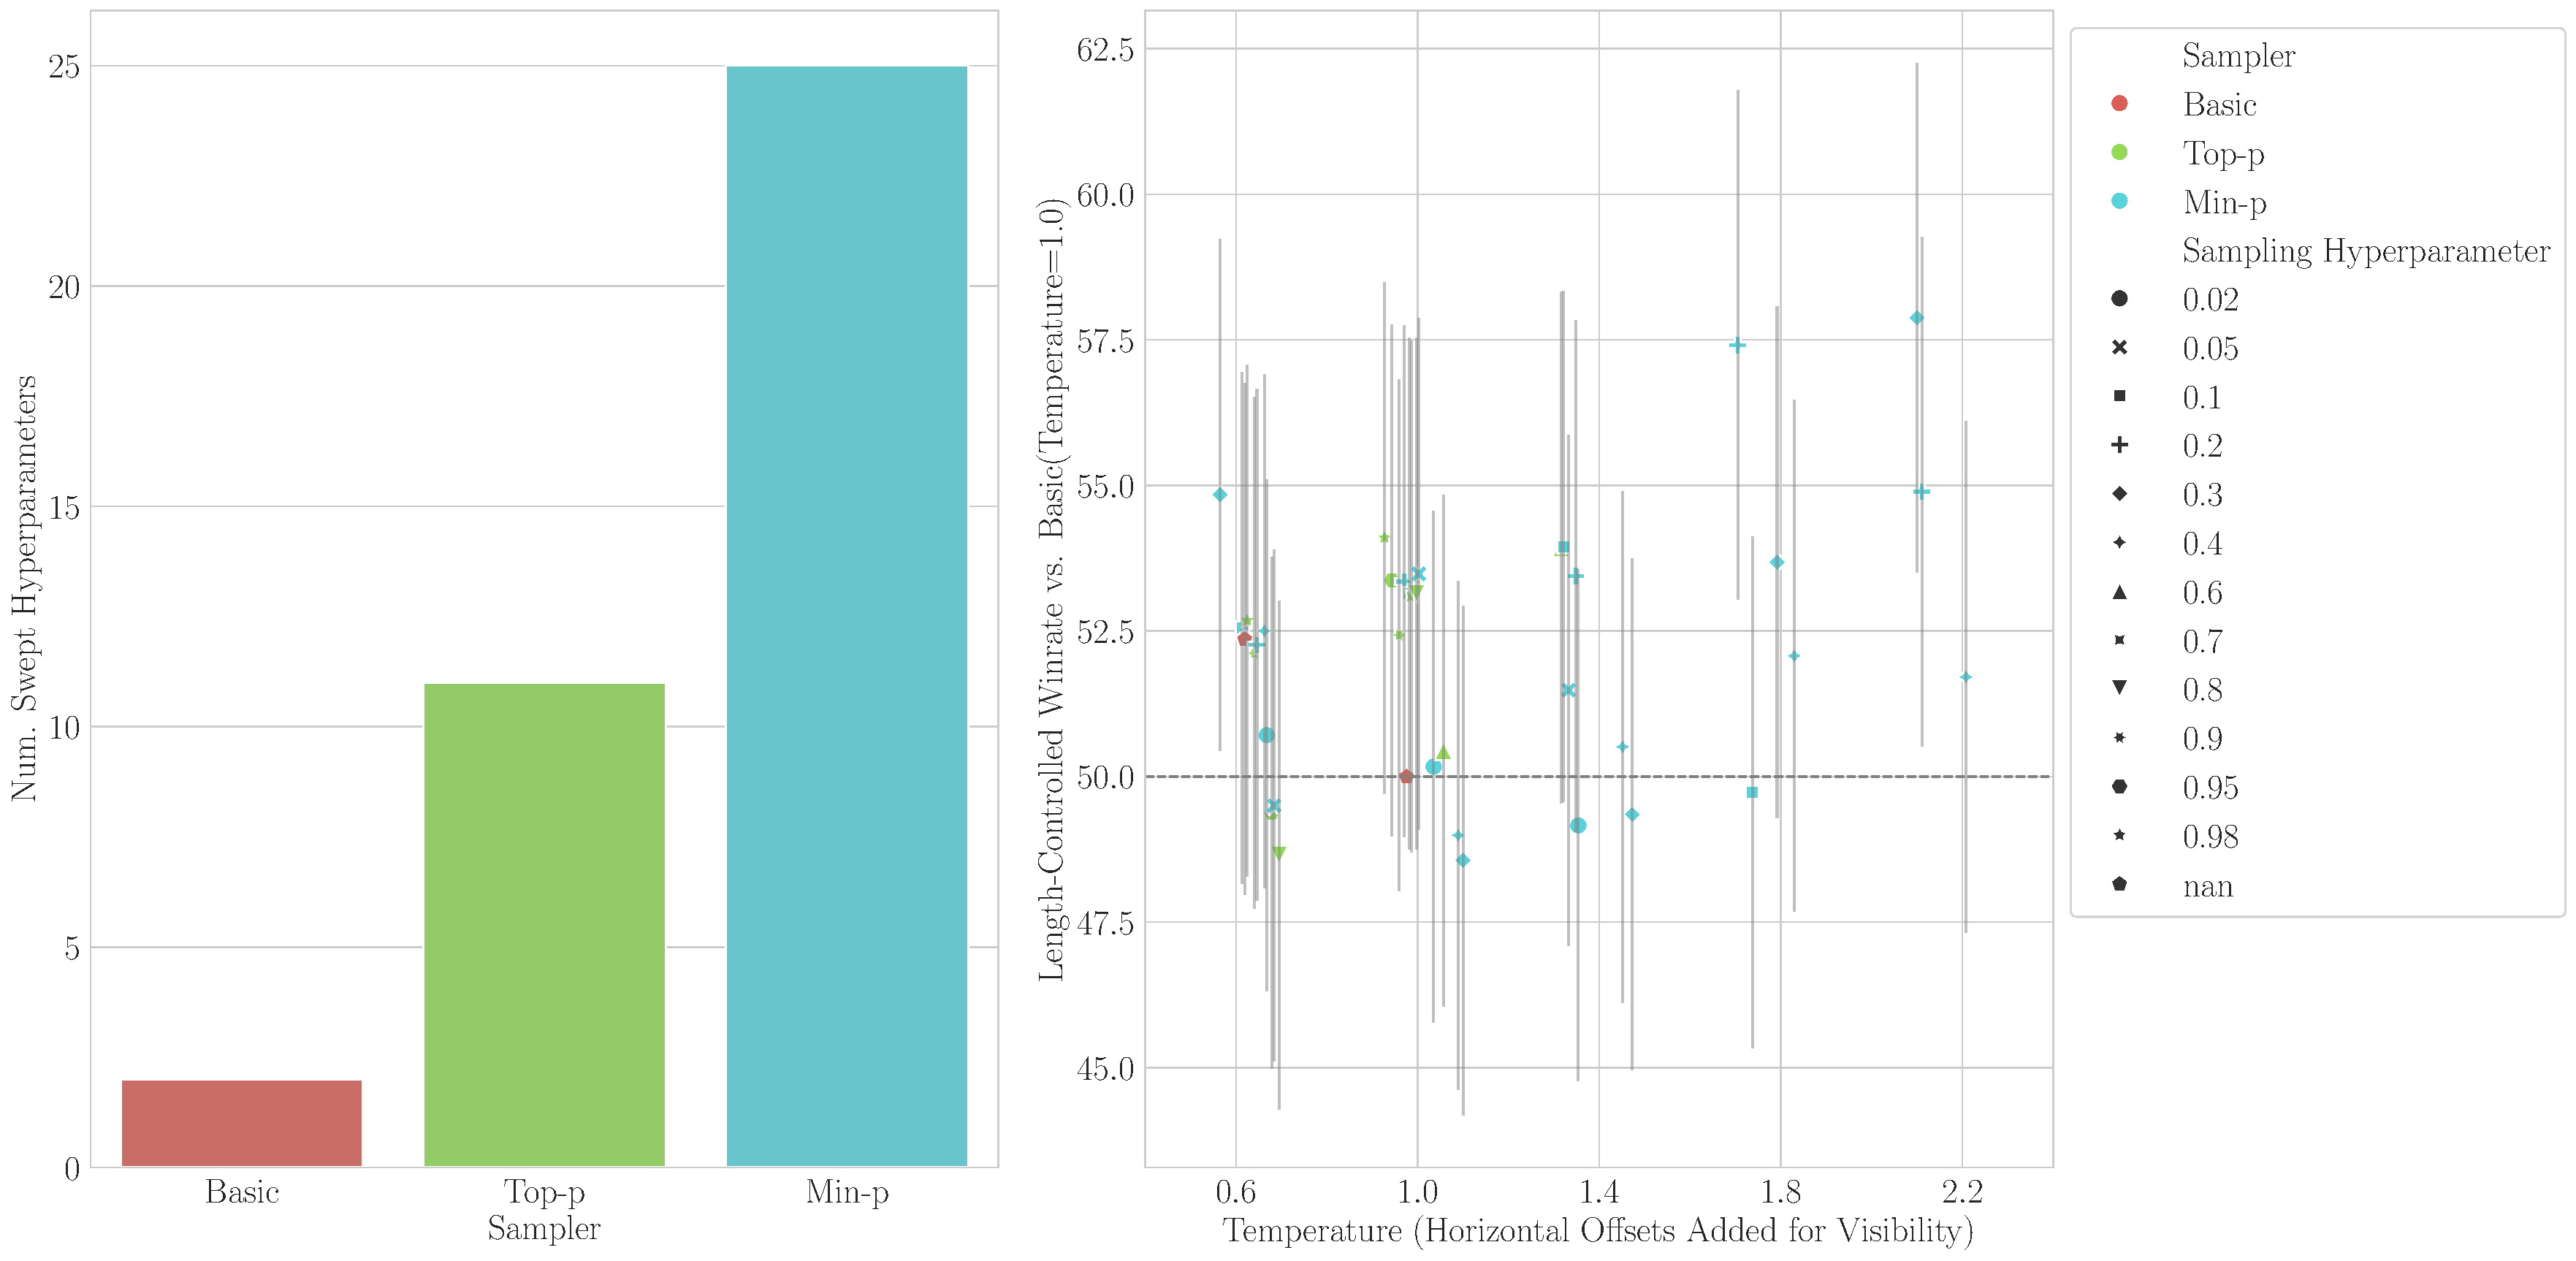
\includegraphics[width=0.9\linewidth]{figures/alpacaeval/combined_samplers_performance_plot.pdf}
    \caption{\textbf{\citet{nguyen2024minp}'s LLM-As-A-Judge Evaluations Suggest \texttt{Min-p} Typically Matches Other Samplers Despite $2\times$ to $10\times$ More Hyperparameter Tuning.} Left: \citet{nguyen2024minp} swept \texttt{min-p} with more than twice as many hyperparameters as \texttt{top-p} and more than ten times as many hyperparameters as \texttt{basic}. Right: Pairwise comparisons show \texttt{min-p} typically performs on-par with other samplers. Data were obtained from a \href{https://github.com/menhguin/quest?tab=readme-ov-file}{public GitHub repository}.
    }
    \label{fig:alpacaeval}
\end{figure*}


To evaluate how performant each sampler is, we first averaged over the three sampling seeds and then conducted two variants of our BoN Evaluation Protocol:
\begin{enumerate}
    \item For each sampler, we subsampled an equal number of hyperparameters ranging from $N=1$ to $N=100$ and computed the maximum Exact Match (Strict) score achieved by the sampled subset of size $N$. We repeated this process $150$ times, averaging over the subsampled subsets' scores. This tells us the best possible performance each sampler will likely obtain as its hyperparameter space increases.
    
    \item For $N=1$ to $N=100$, we subsampled $N$ hyperparameters per sampler and computed the difference of the maximum Exact Match (Strict) score achieved by \texttt{min-p} minus the maximum score achieved by any other sampler. We repeated this process $150$ times, averaging over the subsampled subsets. This tells us by how much \texttt{min-p} outperforms all other samplers, controlling for hyperparameter volume.
\end{enumerate}


\textbf{Both analyses reached consistent results: \texttt{min-p} does not outperform other samplers when equalizing the volume of hyperparameter space.}
Fig.~\ref{fig:gsm8k_em_strict} and Fig.~\ref{fig:gsm8k_diff_of_em_strict} respectively demonstrate that min-p is largely indistinguishable from other samplers.
We also addressed potential confounds regarding prompt formatting. After sharing these results with the original authors, they noted that their public code defaulted to non-standard prompt formatting; we therefore re-ran the entire sweep using \href{https://github.com/EleutherAI/lm-evaluation-harness/blob/main/lm_eval/tasks/gsm8k/gsm8k-cot.yaml}{standard formatting of GSM8K CoT prompts}. The results (Appendix \ref{app:sec:gsm_cot_scores}) were nearly identical: \texttt{min-p} produced marginally higher scores for only 2 of 12 language models, a result indistinguishable from noise. These findings underscore that \texttt{min-p}'s reported dominance in prior work was likely an artifact of comparing a tuned method against sub-optimally tuned baselines.

\paragraph{Fair Comparison on LLM-As-A-Judge Evaluations}

Closely scrutinizing \href{https://github.com/IlyaGusev/quest/compare/main...menhguin:quest:main}{the authors' LLM-As-A-Judge evaluations} revealed two more insights: (1) \texttt{min-p} received $\mathord{\sim}2\times$ more hyperparameter tuning than \texttt{top-p} and $\mathord{\sim}10\times$ more tuning than \texttt{basic} (Fig.~\ref{fig:alpacaeval}, left), potentially tilting the scales in its favor. (2) the win-rates show that \texttt{min-p} frequently fails to outperform \texttt{top-p} and \texttt{basic}, especially when accounting for confidence intervals; we visualized the new data with 95\% confidence intervals (with horizontal offsets added for visibility) (Fig.~\ref{fig:alpacaeval}, right).

